	
\documentclass[12pt,a4paper, twosite]{article}





%\def\numberdoc{\@title} 

%\ifx\conditionmacro\undefined
%\immediate\write18{%
%	pdflatex --jobname="\numberdoc"
%	"\gdef\string\conditionmacro{1}\string\input\space\jobname"
%}%
%\expandafter\stop
%\fi
\usepackage{multirow}
\usepackage{lmodern}
\usepackage[utf8]{inputenc}
\usepackage[T1]{fontenc}
\usepackage{graphicx}
\usepackage{grffile}
\usepackage{longtable}
\usepackage{wrapfig}
\usepackage{rotating}
\usepackage[normalem]{ulem}
\usepackage{amsmath}
\usepackage{textcomp}
\usepackage{amssymb}
\usepackage{capt-of}
\usepackage{hyperref}
\usepackage[left=2.00cm, right=2.50cm, top=2.50cm, bottom=2.00cm]{geometry}
\usepackage{fancyhdr}
\usepackage{colortbl}
\usepackage{xcolor}
\usepackage[spanish]{babel}
\fancyhead[RO,LE]{\thepage}
\fancyhead[LO]{\emph{\uppercase{\leftmark}}}
\fancyfoot{}
\renewcommand{\headrulewidth}{1.0pt}
\pagestyle{fancy}
\date{\today}

\author{Gastón Valdez \\ gaston.cb.90@gmail.com}
\title{Telemetría y sistema de posicionamiento de antena para interferometría }
\definecolor{titDesc}{HTML}{1194D5}
\definecolor{rowMain}{HTML}{80A0E5}
\definecolor{row1}{HTML}{8FADEE}
\hypersetup{
	pdfborder={0 0 0},
	pdfauthor={Gastón Valdez},
	pdftitle={Reqerimientos de ingenieria de software},
	pdfkeywords={Requerimientos, posicionador de antena},
	pdfsubject={hola mundo},
	pdfcreator={Emacs 26.2 (Org mode 9.1.9)}, 
	pdflang={Spanish}
}


\begin{document}
\begin{titlepage}
\maketitle 
\centering \LARGE Especificación de requerimientos de software. 

\end{titlepage}

\section*{Historial de cambios  }
\begin{tabular}{|c|c|c|}
\hline 
Revisión & Detalles de cambios & Fecha  \\ \hline
A & Creación del documento & 17/3/2022 \\ \hline
B & Corrección de requerimientos &10/4/2022 \\ \hline
C & Se añaden dos requerimientos por pedido del director & 11/4/2022\\ \hline 
D & Entrega de documentación a la catedra de IdS & 11/4/2022 	\\ \hline 
E & Se agregan casos de uso & 12/4/2022 	\\ \hline 
F & Entrega a cátedra de IdS  & 14/4/2022 	\\ \hline 
E & Segunda entrega a cátedra de IdS  & 5/6/2022 	\\ \hline 

\end{tabular}



\newpage
	\tableofcontents	
\newpage
	\section{Introducción}
	\label{sec:org60390fa}
	En este trabajo aún existen incertezas con respecto a la elección del SBC. Esta situación crea requerimientos incompletos y la conexión de los periféricos con el SBC no se han definido, por este motivo esta definición no se encuentra dentro de los requerimientos de interfaces. 
	\subsection{Propósito}
	\label{sec:org434c3ef}
	Este documento presenta la especificación de SRS para el sistema de  posicionamiento de antena del IAR. Este dispositivo generalmente se conoce como rotador, de dos grados de libertad, uno denominado azimuth y otro altura o elevación.  
	Esta dirigido a desarrolladores de software dentro de la institución y a los responsables del área de observatorio y transferencia de tecnología dentro de la institución, quienes son los responsables de la aprobación del proyecto. 
%	Esta dirigido a técnicos y profesionales que validen los requerimientos de software dentro del Instituto Argentino de Radioastronomía. 
	
	
	\subsection{Ámbito del sistema}
	\label{sec:org12e44a1}
	Este sistema es un subsistema del interferómetro MIA [\ref{ref:MIA}] y el proyecto de construcción de estaciones terrenas. El objetivo es realizar el apuntamiento de radiofuentes, y el seguimiento de satelites en forma automática.  El nombre del sistema rotador sera ROT\_IAR. el diseño del subsistema ROT\_IAR deberá ser escalable para una posterior etapa de producción.
	
	
	\subsection{Definiciones, Acrónimos y Abreviaturas}
	\label{sec:orgb158e36}
	\begin{enumerate}
		\item IAR: instituto Argentino de Radioastronomía.  
		\item SRS: Especifición de requerimientos de software.  
		\item EP: Electrónica de potencia.
		\item SBC: Single Board Computer.
		\item TBC: Falta de confirmación.
		\item TBD: Aún no definido.
		\item IdS: Ingeniería de software.
		\item SSI: Single Serial interface.
		
		\item N/A: No aplica.  
	
		  
		
	\end{enumerate}
	
	
	
	\subsection{Referencias}
	\label{sec:org62711e0}
	\begin{enumerate}
		\item \label{ref:MIA}https://www.iar.unlp.edu.ar/slider/observatorio/
		\item \label{ref:ptr} Plan de trabajo CESE.
		\item \label{ref:ptr} IAR-OBS-MIA-REQ-R05 (documento interno).
\end{enumerate}
	
	\subsection{Visión general del documento}
	\label{sec:orgdaca22c}
	
	Este documento se realiza siguiendo el estándar IEEE Std. 830-1998 de acuerdo con los lineamientos de la 
	materia Ingeniería de Software de la carrera de especialización de sistema embebidos.
	
	
	\section{Descripción general del documento}
	\label{sec:orgc1c4017}
	
	\subsection{Perspectiva del producto}
	\label{sec:org24980a8}
%	El proyecto aquí especificado es independiente de otros sistemas y no tiene relación con otros productos
	El software es parte de un sistema mayor y común a dos proyectos: MIA y estaciones terrenas. Este sistema de apuntamiento, se adicionara al sistema mecánico de la antena que esta en fase de construcción. El sistema realiza el apuntamiento de antena y podrá ser automático o manual. El diagrama en bloques del sistema se muestra en la figura \ref{fig:diagramaBloques}. 
	
	 El presente documento describe los requerimientos de software del bloque single board computer(TBD), y las interfaces del sistema que se observa en la figura  \ref{fig:diagramaBloques}. 
	\begin{figure}[h!]
		\centering
		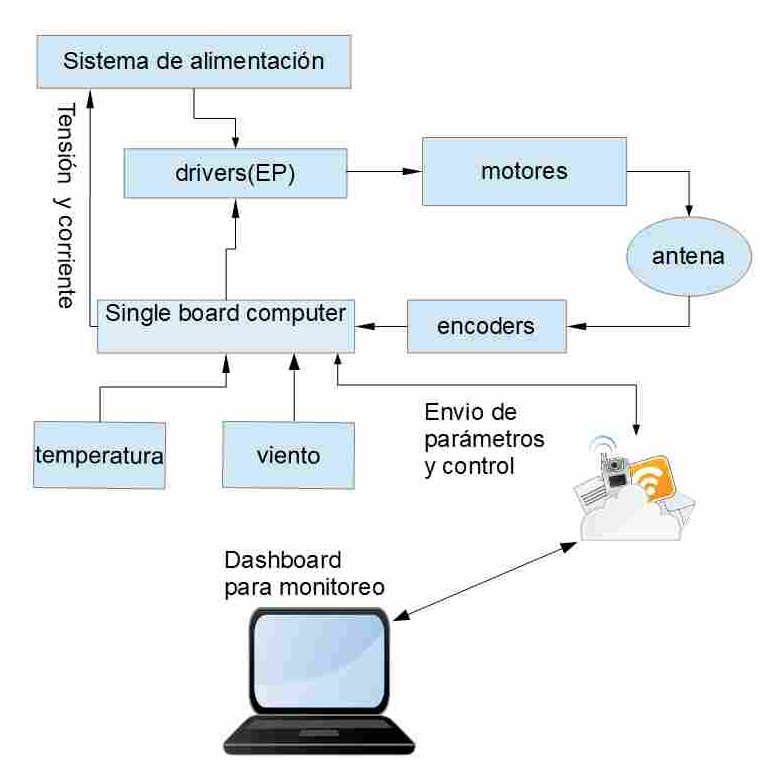
\includegraphics[scale=0.5]{bloquesInt.jpg}
		\caption{Diagrama en bloques del sistema}
		\label{fig:diagramaBloques}
	\end{figure}
	\subsection{Funciones del producto}
	\label{sec:orgaf51da6}
	\begin{enumerate}
		\item Control de posición.
		\item Servidor web embebido. 
		\item Compatible con el software Gpredict y Stellarium, y scripts de antenas principales. 
		\item Reinicio del single board computer en forma remota(TBC).  
		\item Interrupción de operación en caso de condiciones climáticas adversas. 
		\item Información de la operación y estado actual del sistema(tracking, untracked, y cenit). 
	\end{enumerate}
	
	\subsection{Características de los usuarios}
	\label{sec:orga40b0ee}
	Los usuarios serán técnicos, operarios y profesionales con conocimiento y experiencia en los sistemas de apuntamiento y manejo de rotadores. 
	\subsection{Restricciones}
	\label{sec:org5ca5790}
	
	
	\begin{itemize}
		
		\item Lenguaje python 3 para guardar compatibilidad con los scripts de manejo principal de las antenas Carlos Varsavsky y Esteban Bajaja(\ref{ref:MIA}).
		\item El software debe estar bajo control de versiones.  
		\item La documentación se corresponderá con el formato del IAR y con el sistema de numeración del mismo.  
		
%		\item  se debe realizar un informe de avance por cada requerimiento que se cumple 
	\end{itemize}
	
	
	\subsection{Suposiciones y dependencias}
	\label{sec:org0ae23fe}
	\begin{enumerate}
	\item Se supone que se cuenta con los scripts del manejo de las antenas principales.
	\item	Se cuenta con los encoders y motores seleccionados.
	\end{enumerate}
	
	
	
	\subsection{Requisitos futuros}
	\label{sec:org33cfcdb}
	El sistema posea control de velocidad 
	
	El diseño electrónico escalable y realizable en una cadena de producción.  
	
	El sistema debe poseer autocalibración en base al sol o la luna (esto dependerá del horario en que se realice la autocalibración).  
	
	El sistema tendrá que identificarse mediante algún código alfanumérico para brindar sistema de reconocimiento en técnicas de interferometría. 
	
	
	\section{Requisitos específicos}
	\label{sec:org40573d1}
	
	
	\subsection{Interfaces externas}
	\label{sec:orgfd5391f}
	\begin{itemize}
		\item El sistema se comunicara con una red local mediante cable ethernet con conector RJ45[IAR-OBS-MIA-INT-REQ0001] .
		\item El sistema se conecta con un sensor de temperatura DHT11 [IAR-OBS-MIA-INT-REQ0002]. 
		\item El sistema se conecta con los drivers de los motores mediante puertos que posean salida PWM. La velocidad,frecuencia, y porcentaje del PWM será determinado por los ensayos correspondientes sobre los motores[IAR-OBS-MIA-INT-REQ0003].  
		\item Los encoders serán conectados en un conversor analogico digital, bus de comunicación (SSI) o decodificador de cuadratura. Este requerimiento está sujeto a disponibilidad del mercado local del Single Board Computer y el encoder seleccionado(TBD)[IAR-OBS-MIA-INT-REQ0004]. 
		\item El sistema de medición del viento se realizará con un anemómetro, y se conectará a un puerto que incorpore un conversor analógico-digital del Single Board Computer [IAR-OBS-MIA-INT-REQ0005]
%		\item Se realizará un PCB que se acople al Single Board Computer mecánicamente con borneras donde se indique mediante serigrafia la conexión de los perifericos. Esta serigrafia será[IAR-OBS-MIA-INT-REQ0006]: 
%		\begin{itemize}
%			\item EP1: motor de azimuth 
%			\item EP2: motor de altura
%			\item ENC1: encoder de azimuth 
%			\item ENC2: encoder de altura 
%			\item VTO: anemómetro 
%			
%		\end{itemize} 
		
	\end{itemize}
	
	\subsection{Funciones}
	\label{sec:org307bb59}
	\subsubsection{Control de posición}
	\begin{enumerate}
		\item El sistema deberá realizar un control a lazo cerrado de la posición (azimuth y altura) mediante la lectura de los encoders cada 100 ms en modo automático. El tiempo de respuesta debe ser menor al tiempo sidereal del objeto a seguir y el error máximo admitido debe ser menor al ancho de haz de antena(TBD)[IAR-OBS-MIA-FNC-REQ0001]. 
		\item Debe  manejar el sistema de coordenadas ecuatorial y altacimutal y realizar las transformaciones matemáticas correspondientes[IAR-OBS-MIA-FNC-REQ0002]. 
		\item El control se realiza mediante un control proporcional, integral y derivativo[IAR-OBS-MIA-FNC-REQ0003]. 
		\item El sistema tiene tres estados[IAR-OBS-MIA-FNC-REQ0004]: 
			\begin{enumerate}
				\item TRACKING: seguimiento de satélite o radiofuente. Debe ser independiente del tipo de fuente a seguir.
				\item UNTRACKING: no se esta realizando ningún tipo de seguimiento. 
				\item CENIT: posición de reposo de la antena.
			\end{enumerate}

	\end{enumerate}
	\subsubsection{Servidor Web embebido}
	\begin{enumerate}
		\item El servidor informa el valor del estado actual(TRACKING, UNTRACKING, CENIT). Además informa el estado de consumo de corriente en ampere[A], tensión de operación en volts[V], viento en km/h y temperatura en grados centigrados. La medición de la temperatura y velocidad del viento es en el ambiente donde se encuentre el sistema[IAR-OBS-MIA-SWE-REQ0001]. 
		\item Debe realizar movimientos de azimuth y altura a demanda del operador. La precisión debe ser mayor al del encoder seleccionado y debe realizarse en unidades angulares de grados. (TBD)[IAR-OBS-MIA-SWE-REQ0002].
%		\item Debe poseer una función de calibración para los encoders e informar su lectura. Esta realiza la puesta a cero del equipo, y corrige los [IAR-OBS-MIA-SWE-REQ0003]. 
		\item Debe poseer función de calibración para los encoders. La función de calibración realiza las siguientes funciones: 
			\begin{itemize}
				\item Setear el cero de cada coordenada, poniendo el cero en el polo norte o sur(a demanda del operador)
				\item Corrección del corrimiento entre la coordenada solicitada y la que genera el rotador. Esta corrección debe realizarse por los movimientos de nutación y precesión de la tierra.  Esta calibración se realiza en conjunto con los equipos de radiofrecuencia. 
				
			\end{itemize} 
		\item Debe poseer mecanismo para la consulta del estados mediante consola/terminal[IAR-OBS-MIA-SWE-REQ0004]. 
		\item Se deben utlizar los scripts de las antenas principales. Estos scripts contienen gran parte de los cálculos astronómicos desarrollados. Se le debe añadir la conexión con el hardware. Esto implica la realización del servidor web en python. Además el IAR tiene todos sus sistemas corriendo bajo este lenguaje[IAR-OBS-MIA-SWE-REQ0005].
		\item Debe poseer mecanismo para realizar el gráfico de tensión,corriente, viento y temperatura, durante los últimos 10 minutos y verse en pantalla[IAR-OBS-MIA-SWE-REQ0006].
	\end{enumerate}

\subsubsection{Conexión con software externo}
	\begin{itemize}
		\item Debe soportar los protocolos de seguimiento Stellarium y Gpredict para realizar seguimientos de radiofuentes o satelites
		\item Se deben utilizar sockets y configuraciones especificas para cada software. 
	\end{itemize}
%Debe soportar ambos protocolos simultaneamente

\subsection{Entorno de operación y mantenimiento}
\begin{enumerate}
	\item El sistema debe realizar la medición de temperatura y viento cada 2 minutos 
	\item Si la velocidad supera los 50 km/h durante diez minutos, debe llevar la antena a su posición de cenit, independientemente de su estado actual. Si estaba en cenit, debe quedarse allí hasta que la velocidad del viento sea inferior a 50 km/h durante al menos 10 minutos[IAR-OBS-MIA-OPM-REQ0001]
	\item Debe almacenar los datos desde las 5AM de un día, hasta las 5AM del día siguiente, cada dos minutos. Además debe enviar la información a un servidor dentro de la institución. Estos datos tienen el siguiente formato[IAR-OBS-MIA-OPM-REQ0002]: 
	\begin{itemize}
		\item timestamp , tensión[V], corriente[A], temperatura[°C] , viento[KM/H], ESTADO, posición\_azimuth,posición\_altura 
	\end{itemize}  
	La hora de envío será las 5 AM de cada día. El nombre del archivo enviado es en formato txt, y posee el siguiente formato de nombre: 
	\begin{itemize}
		\item IAR\_MIA\_FECHA\_ANTENA.txt 
	\end{itemize} 
	\item El archivo debe ser procesado y almacenado en un directorio dentro del repositorio de la institución mediante un script y realizar un análisis de los parámetros que reciben. En caso de anomalía, debe alertar a los operadores mediante el envío de un SMS o mail.  La alerta indica la falla de alguno de los receptores/control de temperatura/etc que estén adosados al sistema de medición de energía electrica. El script debe desarrollarse por cualquier desarrollador de la institución [IAR-OBS-MIA-OPM-REQ0003].
\end{enumerate}

	\subsection{Requisitos de rendimiento}
	\label{sec:org94bc543}
	
	El sistema, debe soportar hasta 20 conexiones simultaneamente. Si esta en estado TRACKING, al conectarse simultaneamente otro operador, debe informarsele que debe esperar que finalice la operación[IAR-OBS-MIA-OTH-REQ0001]. 
	
	\subsection{Restricciones de diseño}
	\label{sec:org49fe900}
	\begin{enumerate}
		
	\item debe realizar el servidor web embebido en python, para tener compatibilidad con los scripts de manejo de las antenas principales de la institución[IAR-OBS-MIA-OTH-REQ0002]. 
%	\item Los encoders deben tener una resolución menor a 0.2º(diez veces menor que el ancho de haz de antena) [IAR-OBS-MIA-OTH-REQ0002]. 
	\end{enumerate}

	\subsection{Atributos del sistema}
	\label{sec:orgd0babc0}
	Debe tener la capacidad de actualizar el software manualmente mediante red local, si se desea agregar otro software aparte de Gpredict y Stellarium (por ejemplo orbitron)
	
\section{Apéndices}
\label{sec:org75cea03}
	
\subsection{caso de uso 1 }
%1989C2 cyan 
\begin{tabular}{|p{0.001\textwidth}|p{0.25\textwidth}|p{0.2\textwidth}|p{0.5\textwidth}|}
\hline 
\rowcolor{row1}  \multicolumn{2}{|c|}{Título} & \multicolumn{2}{|c|}{Descripción} \\ \hline
\rowcolor{titDesc}
  \multicolumn{2}{|c|}{1. Nombre} & \multicolumn{2}{|c|}{Seguimiento de radiofuentes} \\ \hline

 & 1.1. Breve descripción & \multicolumn{2}{p{0.7\textwidth}|}{En este escenario se configura una radiofuente a seguir}  \\ \cline{2-4} 
 & 1.2. Actor Principal & \multicolumn{2}{p{0.7\textwidth}|}{Operadores de antena}  \\ \cline{2-4}  
 &1.3. Disparadores & \multicolumn{2}{p{0.7\textwidth}|}{Estrella o satélite a seguir }  \\ \hline 

%consultar si unir las dos filas ! 
%\columncolor{rowMain}
%\rowcolor{rowMain}
\multicolumn{4}{|>{\columncolor{rowMain}[8pt][19pt]}p{\textwidth}|}{2. Flujo de eventos} \\ \hline 
&2.1. Flujo básico &\multicolumn{2}{p{0.7\textwidth}|}{2.1.1. Elegir programa de apuntamiento (Gpredict,Stellarium o scripts bash)\newline 2.1.2. Selección de la fuente a seguir  \newline 2.1.3. El dispositivo recibe las coordenadas y debe realizar el cálculo del seguimiento\newline 2.1.4. Finaliza el seguimiento \newline 2.1.5. Vuelve a la posición del cenit }  \\ \cline{2-4}  

% consultar si hay que unir las filas 
& 2.2. Flujo alternativo   &  \multicolumn{2}{p{0.7\textwidth}|}{
	2.2.1. El sistema detecta que las coordenadas son erroneas \newline2.2.2. Alerta al operador de la situación 
	\newline2.2.3. Vuelve a la posición del cenit 	
}  \\ \hline  

 
\multicolumn{2}{|p{0.3\textwidth}|}{3. Requerimientos especiales } & 
\multicolumn{2}{|p{0.7\textwidth}|}{ 3.1. El viento no supera los 50 km/h durante toda la operación de seguimiento}  \\ \hline  
\multicolumn{2}{|p{0.3\textwidth}|}{4. Pre-condiciones }  & \multicolumn{2}{p{0.7\textwidth}|}{ 4.1. Estado de UNTRACKING }  \\   
\hline 
\multicolumn{2}{|p{0.3\textwidth}|}{5. Post-condiciones } 
&   \multicolumn{2}{p{0.7\textwidth}|}{5.1. Estado de UNTRACKING}  \\ \hline  

\end{tabular}


\subsection{caso de uso 2 }

\begin{tabular}{|p{0.001\textwidth}|p{0.28\textwidth}|p{0.2\textwidth}|p{0.5\textwidth}|}
	\hline 
	%\rowcolor{red}
	%\multicolumn{4}{|p{\textwidth}|}{} \\ \hline una sola fila en primera columnta 
\rowcolor{row1}	\multicolumn{2}{|c|}{Título} & \multicolumn{2}{|c|}{Descripción} \\ \hline
\rowcolor{titDesc}	\multicolumn{2}{|c|}{1. Nombre} & \multicolumn{2}{|c|}{Vientos superiores a 50 km/h} \\ \hline
	
	& 1.1. Breve descripción & \multicolumn{2}{p{0.7\textwidth}|}{En este escenario se intenta seguir una radiofuente con un viento superior a 50 km/h}  \\ \cline{2-4} 
	& 1.2. Actor Principal & \multicolumn{2}{p{0.7\textwidth}|}{Operadores de antena}  \\ \cline{2-4}  
	&1.3. Disparadores & \multicolumn{2}{p{0.7\textwidth}|}{Estrella o satélite a seguir }  \\ \hline 
	
	%consultar si unir las dos filas ! 

	\multicolumn{4}{|>{\columncolor{rowMain}[7pt][22pt]}p{\textwidth}|}{2. Flujo de eventos} \\ \hline 
	&2.1. Flujo básico &\multicolumn{2}{p{0.7\textwidth}|}{2.1.1. Elegir programa de apuntamiento (Gpredict,Stellarium o scripts bash)\newline 2.1.2. Selección de la fuente a seguir  \newline 2.1.3. El dispositivo recibe las coordenadas e independiente de la precondición vuelve al cenit  \newline 2.1.4. Alerta al operador \newline 2.1.5. Vuelve a la posición del cenit \newline 
	2.1.6. Finaliza la operación }  \\ \cline{2-4}  
	
	% consultar si hay que unir las filas 
	& 2.2. Flujo alternativo   &  \multicolumn{2}{p{0.7\textwidth}|}{
	2.2.1. El sistema no puede volver al cenit \newline 
	2.2.2. Debe volver manualmente al cenit (sistema manual) }  \\ \hline  
	
	
	\multicolumn{2}{|p{0.3\textwidth}|}{3. Requerimientos especiales } & 
	\multicolumn{2}{p{0.7\textwidth}|}{ 3.1 El sistema debe estar encendido al menos 10 minutos.}  \\ \hline  
	\multicolumn{2}{|p{0.3\textwidth}|}{4 Pre-condiciones }  & \multicolumn{2}{p{0.7\textwidth}|}{ 4.1. Estado de UNTRACKING o TRACKING }  \\   
	\hline 
	\multicolumn{2}{|p{0.3\textwidth}|}{5. Post-condiciones } 
	&   \multicolumn{2}{p{0.7\textwidth}|}{5.1. Estado de CENIT}  \\ \hline  

\end{tabular}


\subsection{caso de uso 3 }


\begin{tabular}{|p{0.001\textwidth}|p{0.28\textwidth}|p{0.2\textwidth}|p{0.5\textwidth}|}
	\hline 
	%\rowcolor{red}
	%\multicolumn{4}{|p{\textwidth}|}{} \\ \hline una sola fila en primera columnta 
\rowcolor{row1}	\multicolumn{2}{|c|}{Título} & \multicolumn{2}{|c|}{Descripción} \\ \hline
\rowcolor{titDesc}	\multicolumn{2}{|c}{1. Nombre} & \multicolumn{2}{|c|}{Al menos dos operadores con conexión a la antena } \\ \hline
	
	& 1.1. Breve descripción & \multicolumn{2}{p{0.7\textwidth}|}{Dos operadores intentan realizar movimientos sobre la antena al mismo tiempo}  \\ \cline{2-4} 
	& 1.2. Actor Principal & \multicolumn{2}{p{0.7\textwidth}|}{Operadores de antena}  \\ \cline{2-4}  
	&1.3. Disparadores & \multicolumn{2}{p{0.7\textwidth}|}{Estrella o satélite a seguir }  \\ \hline 
%\rowcolor{rowMain}	
	\multicolumn{4}{|>{\columncolor{rowMain}[8pt][22pt]}p{\textwidth}|}{2. Flujo de eventos} \\ \hline 
	&2.1. Flujo básico &\multicolumn{2}{p{0.7\textwidth}|}{2.1.1. Detectar que operador solicitó primero el movimiento de la antena \newline 
	2.1.2. Cargar en una lista de espera y avisar al segundo operador de esta situación \newline	
	2.1.3. Mover la antena y realizar el seguimiento de este operador \newline
	2.1.4. Al finalizar el primer seguimiento verificar si es posible satisfacer el segundo
	 \newline
	2.1.5. Si es posible realizar el segundo seguimiento debe realizarlo, en caso contrario debe volver la antena al cenit\newline
	2.1.6. Si no es posible realizar el segundo seguimiento debe volver la antena al cenit}  \\ \cline{2-4}  
	% consultar si hay que unir las filas 
	& 2.2. Flujo alternativo   &  \multicolumn{2}{p{0.7\textwidth}|}{
		N/A
	}  \\ \hline  
	
	\multicolumn{2}{|p{0.3\textwidth}|}{3. Requerimientos especiales } & 
	\multicolumn{2}{p{0.7\textwidth}|}{N/A
	}  \\ \hline  
	\multicolumn{2}{|p{0.3\textwidth}|}{4 Pre-condiciones }  & \multicolumn{2}{p{0.7\textwidth}|}{N/A }  \\   
	\hline 
	\multicolumn{2}{|p{0.3\textwidth}|}{5. Post-condiciones } 
	&   \multicolumn{2}{p{0.7\textwidth}|}{5.1. Estado de UNTRACKING o CENIT}  \\ \hline  
	
\end{tabular}








	
	
\end{document}